Tutti i linguaggi offrono, nella propria libreria standard, un insieme di
strutture dati volte a semplificare la vita ai programmatori implementando
quelli che sono i migliori algoritmi noti per gestire problemi comuni:

\begin{itemize}
  \item Liste ordinate
  \item Insiemi di elementi univoci
  \item Mappe chiave-valore
\end{itemize}

Se esistono strategie diverse di implementazione, spesso sono presenti versioni
alternative con diverse caratteristiche in termini di prestazioni.


È responsabilità del programmatore conoscere le proprietà di complessità delle
diverse strutture dati e riconoscere in quale occasione sia opportuno utilizzare
l'una piuttosto che l'altra.

\section{Complessità nel tempo}
\begin{table}[h!]
  \renewcommand{\arraystretch}{1.6}
  \centering
  \begin{tabular}{l c c c c}
    \toprule
    \textbf{Descrizione}        & \textbf{Accesso} & \textbf{Ricerca} & \textbf{Inserimento} & \textbf{Cancellazione} \\
    \midrule
    Array dinamico              & $O(1)$           & $O(n)$           & $O(n)$               & $O(n)$                 \\
    Coda a doppia entrata       & $O(n)$           & $O(n)$           & $O(1)$               & $O(1)$                 \\
    Lista doppiamente collegata & $O(n)$           & $O(n)$           & $O(1)$               & $O(1)$                 \\
    Coda a priorità             & $O(1)$           & -                & $O(\log(n))$         & $O(\log(n))$           \\
    Tabella hash                & $O(1)$           & $O(1)$           & $O(1)$               & $O(1)$                 \\
    Mappa ordinata              & $O(\log(n))$     & $O(\log(n))$     & $O(\log(n))$         & $O(\log(n))$           \\
    Insieme Hash                & -                & $O(1)$           & $O(1)$               & $O(1)$                 \\
    Insieme ordinato            & -                & $O(\log(n))$     & $O(\log(n))$         & $O(\log(n))$           \\
    \bottomrule
  \end{tabular}
\end{table}

\clearpage

\begin{sidewaystable}
  \renewcommand{\arraystretch}{1.6}
  \centering
  % Usiamo >{\raggedright\arraybackslash}X per allineare il testo a sinistra 
  % ed evitare che gli spazi vengano tirati in modo innaturale
  \begin{tabularx}{\textwidth}{>{\raggedright\arraybackslash}X
      >{\raggedright\arraybackslash}X
      >{\raggedright\arraybackslash}X
      >{\raggedright\arraybackslash}X
      >{\raggedright\arraybackslash}X}
    \toprule
    \textbf{Descrizione}          & \textbf{Rust}                           & \textbf{C++}                                                                          & \textbf{Java}                                   & \textbf{Python}                        \\
    \midrule
    Array dinamico                & \texttt{std::Vec<T>}                    & \texttt{std::vector<T>}                                                               & \texttt{java.util.\allowbreak ArrayList<T>}     & \texttt{list}                          \\
    Coda a doppia entrata         & \texttt{std::VecDeque<T>}               & \texttt{std::deque<T>}                                                                & \texttt{java.util.\allowbreak ArrayDeque<T>}    & \texttt{collections.\allowbreak deque} \\
    Lista doppiamente concatenata & \texttt{std::LinkedList<T>}             & \texttt{std::list<T>} \footnote{Esiste anche singola: \texttt{std::forward\_list<T>}} & \texttt{java.util.\allowbreak LinkedList<T>}    & ---                                    \\
    Coda a priorità               & \texttt{std::BinaryHeap<T>}             & \texttt{std::priority\_queue\allowbreak<T>}                                           & \texttt{java.util.\allowbreak PriorityQueue<T>} & \texttt{heapq}                         \\
    Tabella hash                  & \texttt{std::HashMap\allowbreak<K, V>}  & \texttt{std::unordered\_map\allowbreak<K, V>}                                         & \texttt{java.util.\allowbreak HashMap<K, V>}    & \texttt{dict}                          \\
    Mappa ordinata                & \texttt{std::BTreeMap\allowbreak<K, V>} & \texttt{std::map<K, V>}                                                               & \texttt{java.util.\allowbreak TreeMap<K, V>}    & ---                                    \\
    Insieme hash                  & \texttt{std::HashSet<T>}                & \texttt{std::unordered\_set\allowbreak<T>}                                            & \texttt{java.util.\allowbreak HashSet<T>}       & \texttt{set}                           \\
    Insieme ordinato              & \texttt{std::BTreeSet<T>}               & \texttt{std::set<T>}                                                                  & \texttt{java.util.\allowbreak TreeSet<T>}       & ---                                    \\
    \bottomrule
  \end{tabularx}
\end{sidewaystable}



\clearpage
\FloatBarrier
\section{Complessità}

\begin{figure}[h!]
  \centering
  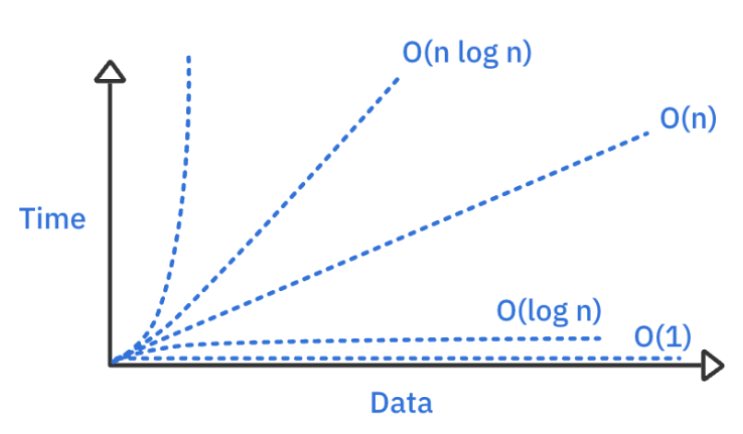
\includegraphics[width=0.3\linewidth]{content/API_Programming/images/2026-04-02-16-51-13.png}
\end{figure}



\section{Metodi comuni a tutte le collezioni}
Tutte le collezioni, messe a disposizione della standard library di Rust,
offrono una serie di metodi comuni tra cui:

\begin{itemize}
  \item \texttt{new()}: alloca una nuova collezione
  \item \texttt{len()}: permette di conoscere l'attuale dimensione della
        collezione
  \item \texttt{clear()}: rimuove tutti gli elementi della
        collezione
  \item \texttt{is\_empty()}: ritorna true se la collezione è vuota
  \item  \texttt{iter()}: per iterare sui valori della collezione

\end{itemize}

Oltre a questi metodi di base, tutte le collezioni implementano i tratti
\texttt{IntoIterator} e \texttt{FromIterator}:

\begin{itemize}
  \item \texttt{into\_iter()}: permette di convertire qualsiasi collezione in un iteratore
  \item \texttt{collect()}:permette di ottenere una collezione partendo da un iteratore
\end{itemize}

\section{Vec<T>}
Il tipo \texttt{Vec<T>} rappresenta una sequenza ridimensionabile di elementi di tipo \texttt{T},
allocati sullo heap. Questa collezione offre una serie di metodi per accedere al
suo contenuto e per inserire/togliere valori al suo interno.

Una variabile di tipo \texttt{Vec<T>} è una tupla formata da tre valori privati:

\begin{itemize}
  \item \texttt{ptr}: Un puntatore ad un buffer allocato sullo
        heap nel quale sono memorizzati gli elementi
  \item \texttt{len}: Un intero privo
        di segno che indica la dimensione complessiva del buffer
  \item \texttt{cap}: Un
        intero privo di segno che indica quanti elementi sono valorizzati nel buffer
\end{itemize}


Se si richiede ad un oggetto di tipo \texttt{Vec<T>} di inserire un nuovo
elemento, questo verrà memorizzato nel buffer nella prima posizione libera e
verrà incrementato il contatore che indica il numero di elementi effettivamente
presenti.

Nel caso in cui il buffer fosse già completo, verrà allocato un nuovo buffer di
dimensioni maggiori. Il contenuto del buffer precedente sarà riversato in
quello nuovo, dove verrà poi anche inserito il nuovo elemento. Dopodiché il
buffer precedente sarà deallocato.

\subsection{Metodi di Vec<T>}
Offre una vasta serie di metodi per accedere al suo contenuto e per
inserire/togliere valori al suo interno, tra cui:


\begin{itemize}
  \item \texttt{Vec::with\_capacity(n)} alloca un vettore con capacità n
  \item \texttt{capacity()} ritorna la lunghezza del vettore
  \item \texttt{push(value)} aggiunge un elemento alla fine del vettore
  \item \texttt{pop()} rimuove e ritorna un \texttt{std::Option} contenente l'ultimo
        elemento del vettore, se esistente
  \item \texttt{insert(index, value)} aggiunge un elemento alla posizione ricevuta in argomento
  \item \texttt{remove(index)} rimuove e ritorna l'elemento alla posizione ricevuta in argomento
  \item ...
\end{itemize}

I dati contenuti in un vettore devono essere omogenei.  Se occorre memorizzare
dati di tipo differente, è possibile utilizzare un tipo enumerativo come busta
per tali elementi

\begin{center}
  \begin{minipage}{0.55\linewidth}
    \begin{minted}[breaklines]{rust}
  let row = vec![
    SpreadsheetCell::Int(3),
    SpreadsheetCell::Text(String::from("blue")),
    SpreadsheetCell::Float(10.12),
    ];
\end{minted}
  \end{minipage}%
  \hfill
  \begin{minipage}{0.4\linewidth}
    \begin{minted}[breaklines]{rust}
  enum SpreadsheetCell {
  Int(i32),
  Float(f64),
  Text(String),
  }
  \end{minted}
  \end{minipage}
\end{center}


\section{VecDeque<T>}
Il tipo \texttt{VecDeque<T>} modella una coda a doppia entrata: esso alloca sullo heap una
serie di elementi di tipo \texttt{T}.

A differenza di \texttt{Vec<T>}, permette l'inserimento e la rimozione, con
costo unitario, sia all'inizio che alla fine del vettore tramite i metodi
\texttt{push\_front()}, \texttt{push\_back()}, \texttt{pop\_front()} e \texttt{pop\_back()}.


Viene implementato come un buffer circolare e non garantisce che gli elementi
siano contigui in memoria, per rendere gli elementi contigui in
memoria utilizzando il metodo

\begin{tcolorbox}
  \textbf{Nota:} \texttt{VecDeque<T>} risulta più veloce di \texttt{Vec<T>} se se
  si eseguono molte \texttt{pop\_front()}. In tutti gli altri casi è preferibile
  utilizzare \texttt{Vec<T>}.
\end{tcolorbox}


\section{LinkedList<T>}

Il tipo \texttt{LinkedList<T>} permette di rappresentare in memoria una lista
doppiamente collegata, il tempo di accesso è costante.

Come per \texttt{VecDeque<T>}, permette di inserire e rimuovere elementi da
entrambe le estremità della lista.

È possibile inizializzare una \texttt{LinkedList<T>} a partire da un array
\mintinline{rust}|let ll = LinkedList::from([1, 2, 3]);|

\subsection{Metodi}

I metodi attualmente offerti da \texttt{LinkedList<T>} sono un ristretto
sottoinsieme dei metodi offerti da \texttt{VecDeque<T>}.

Tuttavia, è quasi sempre preferibile utilizzare \texttt{Vec<T>}  o \texttt{VecDeque<T>}
poiché superiori in termini di prestazioni ed uso della memoria.

\section{Mappe}

\subsection{HashMap<K,V>}

Una \texttt{HashMap<K,V>} è una collezione di coppie composte da una chiave di tipo
\texttt{K} e un valore di tipo \texttt{V}: i valori sono salvati nello
heap come una sinfola hash table.

È preferibile utilizzare una \texttt{HashMap<K,V>} quando le chiavi \textbf{NON} hanno
un ordine. L'inserimento di una nuova entry nella \texttt{HashMap<K,V>} può causare
la riallocazione ed il movimento dei dati.


La chiave deve essere univoca ed il tipo \texttt{K} deve implementare i tratti \texttt{Eq} e \texttt{Hash}.


\subsection{BTreeMap<K,V>}

Una \texttt{BTreeMap<K,V>} è una collezione di coppie composte da una chiave di tipo
\texttt{K} e un valore di tipo \texttt{V}: i valori sono salvati nello
heap come un singolo albero dove ogni entry rappresenta un nodo.

È preferibile utilizzare una \texttt{BTreeMap<K,V>} quando le chiavi hanno un ordine, per
migliorare l'efficienza di accesso ai nodi.

Anche in questo caso l'inserimento di una nuova entry nella \texttt{BTreeMap<K,V>} può causare la riallocazione ed il movimento dei dati.ù

La chiave deve essere univoca ed il tipo \texttt{K} deve implementare il tratto \texttt{Ord}.


\subsection{Mappe e possesso}
Poiché una mappa nella maggior parte dei casi possiede sia le chiavi che i valori
presenti al suo interno, le operazioni relative all'inserimento, cancellazione, accesso
ai singoli elementi richiedono il rispetto di tale possesso.

Inoltre, Rust cerca di ottimizzare l'accesso ai dati contenuti evitando di dover
navigare più volte la struttura interna alla ricerca del valore associato ad un
chiave.



La conseguenza di ciò è che l'interfaccia applicativa offerta è alquanto differente da
quella tipicamente offerta da altri linguaggi, pur avendo lo stesso potere espressivo.

In particolare:


\begin{itemize}
  \item \textbf{Accesso}: i metodi di accesso, \mintinline{rust}|get(...)|, \mintinline{rust}|get_key_value(...)|,
        \mintinline{rust}|keys(...)|, etc., usano chiavi di tipo referenziato, \texttt{\&K},
        e ritornano valori di tipo referenziato, \texttt{\&V}.
  \item \textbf{Modifica}: i metodi che modificano la mappa tendono ad usare riferimenti a chiavi e valori, \mintinline{rust}|remove(...)|, \mintinline{rust}|retain(...)|.
  \item \textbf{Inserimento}: i metodi di inserimento richiedono invece il movimento di valori posseduti
  \item \textbf{Sostituzione}: La sostituzione di un valore avviene presente nella mappa ha un approccio particolare, attraverso il
        concetto di \texttt{Entry}
\end{itemize}


\section{Entry<'a,K,V>}
Rust offre la possibilità di ottimizzare l'utilizzo delle mappe: in particolare attraverso
il metodo \texttt{entry} che permette di cercare una chiave all'interno di una mappa e
ritorna un enum in base al risultato della ricerca

\begin{center}
  \mintinline{rust}|entry(&mut self, key: K) -> Entry<'a, K, V>|
\end{center}

L'enum \texttt{Entry} mette a disposizione diversi metodi per la gestione del
risultato, permettendo di ridurre il numero di spostamenti in memoria:

\begin{itemize}
  \item \mintinline{rust}|and_modify<F>(self, f: F)| in caso di successo
        permette di eseguire delle azioni aggiuntive sul risultato ottenuto
  \item \mintinline{rust}|or_insert(self, default: V)| in caso di fallimento è
        possibile inserire una nuova entry senza costi aggiuntivi poiché il puntatore
        sarà già indirizzato verso una zona di memoria libera
\end{itemize}


\begin{minted}[breaklines]{rust}
let mut animals: HashMap<&str, u32> = HashMap::new();
 animals.entry("dog")
        .and_modify(|e| { *e += 1 })
        .or_insert(1);
\end{minted}


\subsection{Operare con le mappe}

\begin{minted}[breaklines]{rust}
use std::collections::HashMap;

fn main() {
  // inizializzo una mappa a partire da un insieme di valori
  let mut scores = HashMap::from([("Alice",80), ("Bob", 90), ("Carol",70)]);
  // modifico il valore associato ad una chiave
  scores.entry("Carol").and_modify(|v| *v = 75 );
  // trasferisco il contenuto della mappa in un Vec<(K,V)>
  let mut v: Vec<(&'static str, i32)> = scores
  .into_iter()
  .collect();
  // ordino per valore
  v.sort_by_key(|(_, val)| *val);
  println!("{:?}",v);
}
\end{minted}


\section{Insiemi}

\subsection{HashSet<T>}

Un \texttt{HashSet<T>} è un insieme di elementi univoci di tipo \texttt{T} i cui
valori sono salvati nello heap come singole hash table.

\begin{itemize}
  \item L'inserimento di una nuova entry nell'\texttt{HashSet<T>} può causare la riallocazione e il movimento dei dati.
  \item Un \texttt{HashSet<T>} è implementato come un wrapper attorno ad una \texttt{HashMap<T, ()>}
\end{itemize}


\subsection{BTreeSet<T>}

Un \texttt{BTreeSet<T>} è un insieme di elementi univoci di tipo \texttt{T} i cui
valori sono salvati nello heap come un singolo albero dove ogni entry rappresenta un nodo.

\begin{itemize}
  \item L'inserimento di una nuova entry nell'\texttt{BTreeSet<T>} può causare la riallocazione e il movimento dei dati.
  \item Un \texttt{BTreeSet<T>} è implementato come un wrapper attorno ad una \texttt{BTreeMap<T, ()>}
\end{itemize}



\section{BinaryHeap<T>}

Un \texttt{BinaryHeap<T>} è una collezione di elementi di tipo \texttt{T} i cui valori sono salvati nello heap
e l'elemento più grande si trova sempre nella prima posizione.

Il tipo \texttt{T} deve implementare il tratto \texttt{Ord} per poter essere ordinato.

Il metodo \texttt{peek()} permette di ritornare l'elemento più grande con
complessità $O(1)$. Nel caso peggiore, se si modifica l'elemento attraverso il metodo
\texttt{peek\_mut()}, la complessità diventa $O(n)$.



% Opzione 2: La soluzione "Pro" (L'estensione HyperSnips) Se non vuoi fare Ctrl+V
% ma vuoi che il testo si espanda magicamente mentre scrivi, la soluzione
% definitiva si chiama HyperSnips (è un'estensione per VS Code).

% HyperSnips ti permette di usare le Espressioni Regolari (Regex) e il codice
% JavaScript dentro gli snippet.

% Installa l'estensione HyperSnips su VS Code.

% Apri il file degli snippet per LaTeX (tramite comando HyperSnips: Open Snippet
% File -> latex.hsnips).

% Incolla una logica come questa:

% JavaScript snippet `tab(\d+)x(\d+)` "Tabella dinamica" A ``rv =
% "\\begin{table}[h!]\n\\centering\n\\begin{tabular}{" + "c ".repeat(m[2]) +
% "}\n\\toprule\n" for (let i = 0; i < m[1]; i++) { rv += " & ".repeat(m[2]-1) + "
% \\\\\n" } rv += "\\bottomrule\n\\end{tabular}\n\\end{table}"`` endsnippet Come
% si usa: Tu non dovrai aprire nessun form. Mentre scrivi il tuo codice LaTeX,
% digiti semplicemente tab3x4. Appena digiti l'ultimo numero, HyperSnips riconosce
% il pattern, estrae "3" e "4" tramite la Regex, calcola il JavaScript in
% background e ti stampa immediatamente una tabella 3x4 completa al posto di
% "tab3x4". È la cosa più vicina alla magia che si possa ottenere su VS Code.
